

\section{Text entry method}

In the proposal for this project, it was suggested that an interesting way of getting the input text from the user would be to implement a chatbot interface within a web app, using a plugin service to facilitate this. 

There are many platforms available on which chat bots can be built like Slack or WhatsApp, but the decision has been made to look more into Facebook and Microsoft's solutions since these are the ones with the largest amount of documentation.

\subsection{Facebook Bot Platform}

The platform itself offers some basic Natural Language Processing, but primarily the platform is aimed at businesses, below is the entities in input text that the inbuilt NLP can pick up on and separate out:

\begin{center}
\begin{tabular}{ |c| } 
 \hline
  Recognised Categories \\ 
 \hline                        
 Greeting \\
 Thanks \\
 Bye \\
 Date/Time \\
 Amount of Money \\
 Phone numbers \\
 Email address \\
 Distance \\
 Quantity \\
 Temperature \\
 Volume \\
 Location \\
 Duration \\
 URL \\
 Sentiment \\
 \hline
\end{tabular}
\end{center}

The only category that would be used is the sentiment recognition, but during prototyping this could not be made to work, and there seems to be very few examples of projects using this tool.
Since building the sentiment analysis tool is part of this project, the bot platform not offering useful NLP is not disastrous. 
Issues with this platform include limited access to testing tools while developing, until the bot is approved by Facebook itself which can take a long time, so this may not be the best platform to use. 

\subsection{Microsoft Bot Framework using Azure}

Microsoft's Bot Framework can be implemented through Skype \cite{Azure}, and can be linked up with the Microsoft Language Understanding system, LUIS \cite{LUIS}. This system primarily is built for businesses, and attempts to get the input text intent and entities, as shown below.
\begin{center}
\begin{tabular}{ |c|c|c| } 
 \hline
  User Input & Intent & Entities \\ 
 \hline                        
 Book a flight to Seattle & BookFlight & Seattle \\
 When does your store open? & StoreHoursAndLocation & open \\
 Schedule a meeting at 1PM with Bob in Distribution & ScheduleMeeting & 1PM, Bob \\
 \hline
\end{tabular}
\end{center}

This does not have any inbuilt sentiment analysis which isn't an issue since this is being built separately, but prototyping with this framework and using it for past projects has been difficult to set up, and has been slow.

\subsection{An Alternative}

When the use of a chatbot was suggested during the project proposal, there were issues with this idea raised to do with validating the Spotify account through a chat system. 
After more research into the abilities of the chatbot platforms and how the Spotify Authorisation API works, an alternative would be is to not use a chatbot platform at all for user text input.
There appears to be no available way to allow users to log into their Spotify Account through a messaging system, and as shown in Figure \ref{spotify:auth}, the tokens would have to be generated through a web app on a page, and then having to pass it through the third party bot platform is much more work and seems like unnecessary effort. 

\begin{figure}[ht]
\caption{Diagram from the Spotify Documentation showing the authorisation flow for using the Spotify API \cite{spotifyHello}}
\centering
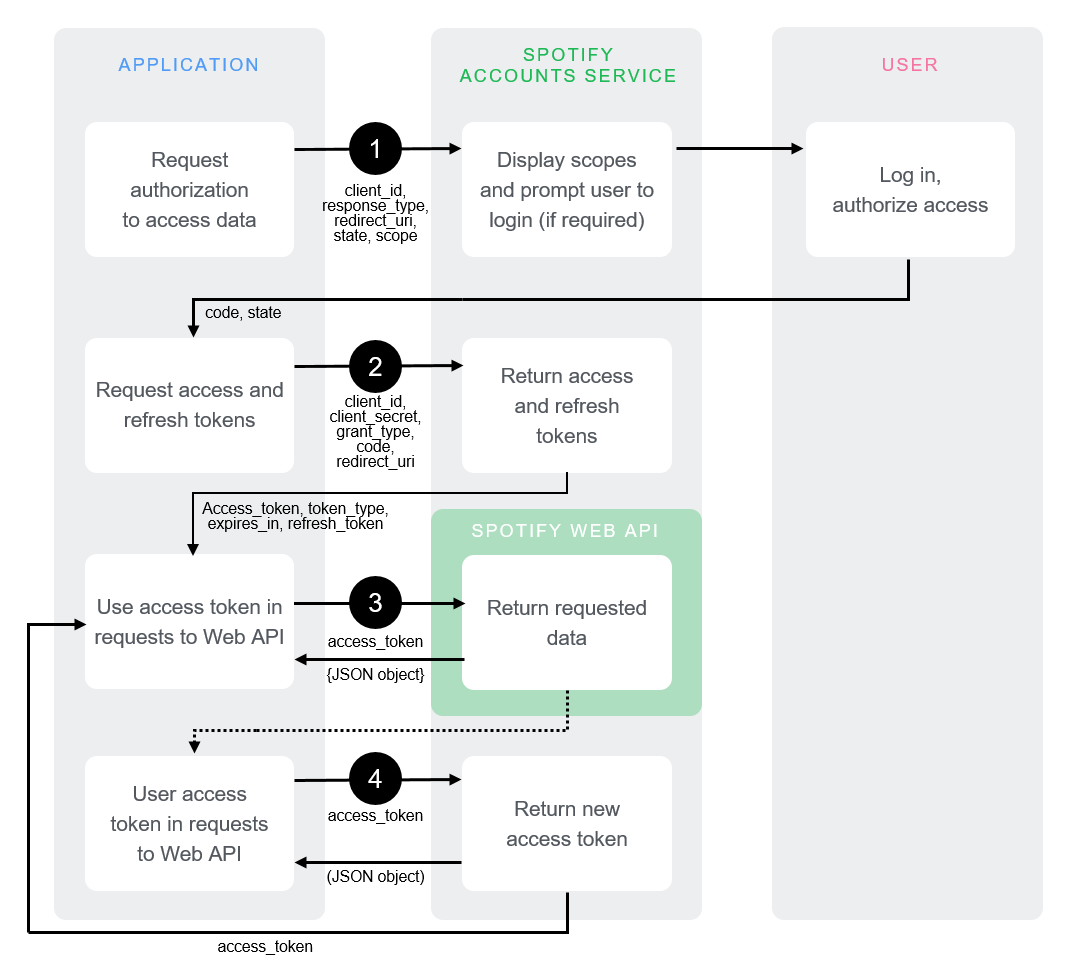
\includegraphics[scale=0.3]{./LitReview/images/spotifyAuthGuide.png}
\label{spotify:auth}
\end{figure}

An alternative would be to have a web application with a forms interface, allowing text box entry. This would still serve exactly the same purpose with easier implementation from a development point of view, since there will be no going through a third party. 
The prompts for emotive user input text can still change and be relevant as logic can be implemented within the web application on the front end with JavaScript. 

After this research into the chatbot platforms, the conclusion has been made that using this method for data input is unnecessarily complex, doesn't add much and would cause issues for the more important part of the project, which is the Spotify API integration. As shown in Figure \ref{programFlow}, the project will be restructured, with the text being input through the use of a forms system on the web application.

\begin{figure}[h]
\caption{The new structure of the project}
\centering
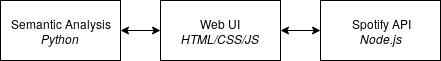
\includegraphics[scale=0.5]{./LitReview/images/ProgramFlow.png}
\label{programFlow}
\end{figure}